\subsection{Implementering af spændingsforsyning}
For at opfylde kravene, der er specificeret i \autoref{sec:krav_spaending}, vælges det at benytte en færdigudviklet komponent, som består af to batterier på $1,5~V$, der sidder i en spændingsregulator. Batteriernes kobling danner et split supply, og derfor dannes der en jordforbindelse fra det ene batteris negative pol og den andens positive pol. De andre poler, som ikke anvendes til jordforbindelse, benyttes som systemets positive spændingsforsyning, ${V}_{cc}$ og negative spændingsforsyning, ${V}_{dd}$.
Spændingsregulatoren sørger for at give en jævn spænding på henholdsvis $3,4~V$ og $\pm 5,5~V$. Dette gøres ved, at spændingsregulatoren oplagrer spænding fra de to tilkoblede batterier i spoler, når switchfunktionen lukkes. Switchfunktionen åbnes, når spolerne er mættede og en spænding ledes videre i kredsløbet via en diode. Denne switchfunktion åbner og lukker skiftevis i kort tid, hvilket resulterer i, at en konstant spænding ledes til systemet hele tiden. På sigt vil systemet ikke fungere optimalt, da batterierne ikke vil være i stand til at levere en jævnspænding på grund af levetiden. Spændingsregulatoren vil derfor gøre opmærksom på dette ved at få en LED til at blinke, når der ikke leveres en konstant spænding. 
Konfigurationen af spændingsforsyningen fremgår af \autoref{fig:spaendingsforsyning}, hvor terminalerne for $\pm 5,5~V$ fremgår som rød(V+) og blå(V-) og sort(Gnd), mens der på den modsatte side fremgår terminalerne for $3,4~V$ som brun(Vcc) og sort(Gnd). 

\begin{figure}[H]
\centering
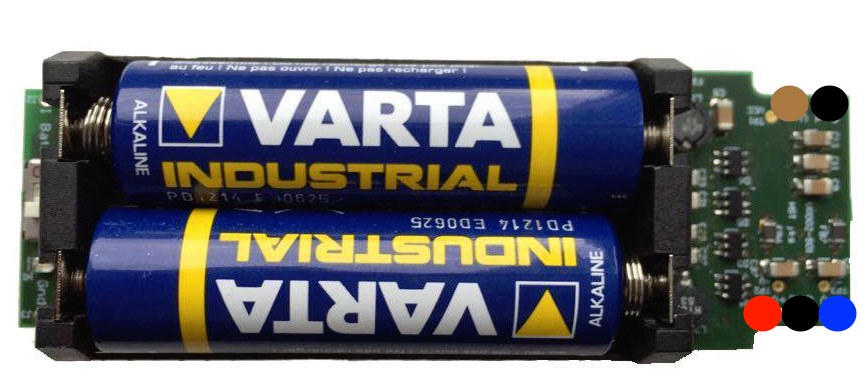
\includegraphics[width=0.5\textwidth]{figures/spaendingsforsyning}
\caption{Spændingsforsyning, der består af to $1,5~V$ batterier i et split supply. Den røde prik illustrerer V+, den blå V-, den sorte Gnd og den brune Vcc.}
\label{fig:spaendingsforsyning}
\end{figure}

